\documentclass[12pt]{article}

% Layout.
\usepackage[top=1.2in, bottom=0.75in, left=1in, right=1in, headheight=1.0in, headsep=0pt]{geometry}

% Fonts.
\usepackage{mathptmx}
\usepackage[scaled=0.86]{helvet}
\renewcommand{\emph}[1]{\textsf{\textbf{#1}}}

% TiKZ.
\usepackage{tikz, pgfplots}
\usetikzlibrary{calc}
\pgfplotsset{my style/.append style={axis x line=middle, axis y line=middle, xlabel={$x$}, ylabel={$y$}}}
\pgfplotsset{compat=1.16}

% Misc packages.
\usepackage{amsmath,amssymb,latexsym,bm,array,multicol,enumitem}
\usepackage{graphicx}
\usepackage{xcolor}

% Commands to set various header/footer components.
\makeatletter
\def\doctitle#1{\gdef\@doctitle{#1}}
\doctitle{Use {\tt\textbackslash doctitle\{MY LABEL\}}.}
\def\docdate#1{\gdef\@docdate{#1}}
\docdate{Use {\tt\textbackslash docdate\{MY DATE\}}.}
\def\doccourse#1{\gdef\@doccourse{#1}}
\let\@doccourse\@empty
\def\docscoring#1{\gdef\@docscoring{#1}}
\let\@docscoring\@empty
\def\docversion#1{\gdef\@docversion{#1}}
\let\@docversion\@empty
\makeatother

% Headers and footers layout.
\makeatletter
\usepackage{fancyhdr}
\pagestyle{fancy}
\fancyhf{} % Clears all headers/footers.
\lhead{\emph{\@doctitle\hfill\@docdate} \medskip
\ifnum \value{page} > 1\relax\else\\
\emph{Name: \rule{3.5in}{1pt}\hfill \@docscoring}
\fi}

\rfoot{\emph{\@docversion}}
\lfoot{\emph{\@doccourse}}
\cfoot{\emph{\thepage}}
\renewcommand{\headrulewidth}{0pt}%
\makeatother

% Paragraph spacing
\parindent 0pt
\parskip 6pt plus 1pt

% A problem is a section-like command. Use \problem{5} for a problem worth 5 points.
\newcounter{probcount}
\newcounter{subprobcount}
\setcounter{probcount}{0}

\newcommand{\problem}[1]{%
\par
\addvspace{4pt}%
\setcounter{subprobcount}{0}%
\stepcounter{probcount}%
\makebox[0pt][r]{\emph{\arabic{probcount}.}\hskip1ex}\emph{[#1 points]}\hskip1ex}

\newcommand{\thesubproblem}{\emph{\alph{subprobcount}.}}

% Subproblems are an enumerate-like environment with a consistent
% numbering scheme.  Use \begin{subproblems}\item...\item...\end{subproblems}
\newenvironment{subproblems}{%
\begin{enumerate}[itemindent=8pt,leftmargin=0pt]%
\setcounter{enumi}{\value{subprobcount}}%
\renewcommand{\labelenumi}{\emph{\textsl{\alph{enumi})}} \,}%
}%
{%
\setcounter{subprobcount}{\value{enumi}}%
\end{enumerate}%
}

% Blanks for answers in normal and math mode.
\newcommand{\blank}[1]{\rule{#1}{0.75pt}}
\newcommand{\mblank}[1]{\underline{\hspace{#1}}}
\def\emptybox(#1,#2){\framebox{\parbox[c][#2]{#1}{\rule{0pt}{0pt}}}}

% Misc.
\renewcommand{\d}{\displaystyle}
\newcommand{\ds}{\displaystyle}
\newcommand{\threeopts}{{\small \hspace{-6mm} $\begin{matrix} \text{\textsc{converges}} \\ \text{\textsc{absolutely}} \end{matrix}$ \qquad\qquad $\begin{matrix} \text{\textsc{converges}} \\ \text{\textsc{conditionally}} \end{matrix}$ \qquad\qquad \textsc{diverges}} \bigskip}

\newcommand{\ba}{\mathbf{a}}
\newcommand{\bb}{\mathbf{b}}
\newcommand{\bc}{\mathbf{c}}
\newcommand{\bi}{\mathbf{i}}
\newcommand{\bj}{\mathbf{j}}
\newcommand{\bk}{\mathbf{k}}
\newcommand{\bn}{\mathbf{n}}
\newcommand{\br}{\mathbf{r}}
\newcommand{\bu}{\mathbf{u}}
\newcommand{\bv}{\mathbf{v}}
\newcommand{\bw}{\mathbf{w}}

\newcommand{\bT}{\mathbf{T}}

\newcommand{\grad}{\nabla}
\newcommand{\Div}{\nabla\cdot}

\newcommand{\ip}[2]{\mathrm{\left<#1,#2\right>}}
\newcommand{\vv}[2]{\mathrm{\left<#1,#2\right>}}
\newcommand{\vvv}[3]{\mathrm{\left<#1,#2,#3\right>}}


\newcommand{\boxy}[1]{\fbox{\Huge \strut \hspace{#1mm} \strut}}
\newcommand{\boxycontent}[2]{\fbox{\quad {\large #2} {\Huge \strut \hspace{#1mm} \strut}}}



\doctitle{\hspace{-6mm} Math 302 Differential Equations: \,{\large Quiz 4}}
\docdate{1 November 2023}
\doccourse{}
\docversion{}
\docscoring{\fbox{{\LARGE \strut}\hspace{0.8in} / 25}}


\begin{document}
$\boxed{35}$ minutes maximum.  No aids (book, calculator, etc.) are permitted.  Show all work; use proper notation for full credit.  Answers should be in reasonably-simplified form.  25 points possible.

% like 4.4 #28, but easier
\problem{8}  Solve the following initial value problem:
	$$y''+5 y' + 4y = 4x + 5, \quad y(0)=0, \, y'(0)=0$$
\vfill
\hfill\boxycontent{90}{$y(x)=$}

\clearpage\newpage
% exactly 5.1 # 6
\problem{9}  A force of 400 Newtons stretches a spring 2 meters.  A mass of 50 kilograms is attached to the end of the spring and then is initially released from from the equilibrium position with an upward velocity of 10 m/s.

\begin{subproblems}
\item The above describes an undamped mass-spring system.  Find the equation of motion.
\vfill
\hfill\boxycontent{90}{$x(t)=$}

\item Suppose we add a damping force $-250\,dx/dt$, that is, with $\beta=250$.  What is the new differential equation?  Find the general solution; you may ignore the initial conditions for this part.
\vfill
\hfill\boxycontent{100}{$x(t)=$}

\item Going back to the undamped mass-spring system in part \textsl{\emph{a)}}, suppose we apply an external force $f(t)=50 e^{-3t}$.  Find the general solution; again you may ignore the initial conditions for this part.
\vfill
\hfill\boxycontent{100}{$x(t)=$}
\end{subproblems}


\clearpage\newpage
% conceptual on 4.4
\problem{8}  Recall the rules for a 2nd-order, linear, constant-coefficient, and homogeneous differential equation
	$$a y'' + b y' + c y = 0$$
which has auxiliary equation $am^2+bm+c=0$ from substituting $y(x)=e^{mx}$.
\renewcommand{\labelenumi}{\textsl{(\roman{enumi})}}
\begin{enumerate}
\item If the roots $m_1,m_2$ of the auxiliary equation are real then \, $y(x) = c_1 e^{m_1 x} + c_2 e^{m_2 x}$.
\item If the root $m_1=m_2$ of the auxiliary equation is repeated then \, $y(x) = c_1 e^{m_1 x} + c_2 x e^{m_1 x}$.
\item If the roots $m_1=\alpha+i\beta,\,m_2=\alpha-i\beta$ of the auxiliary equation are complex then

$y(x) = c_1 e^{\alpha x} \cos(\beta x) + c_2 e^{\alpha x} \sin(\beta x)$.
\end{enumerate}

\begin{subproblems}
\item Explain in two or more sentences which part of the above rules is justified by the reduction of order technique.  Be as specific as you can about how the reduction of order calculation starts, and what it yields, but don't worry about the whole calculation.
\vfill

\item Explain in two or more sentences which part of the above rules is justified by Euler's identity for complex numbers.  In particular, write down Euler's identity.
\vfill
\end{subproblems}


\clearpage\newpage
% xx
\noindent \emph{Extra Credit. [2 point]} \, Find a solution of the DE
    $$ax^2y'' + bxy' + cy = 0$$
of the form $y=x^m$.  (\textsl{Assume you are working on the interval $(0,\infty)$, where $x$ is never zero.})  Show there are in fact two linearly-independent solutions of that form if $(b-a)^2 - 4 a c > 0$.
\vfill

%\centerline{\footnotesize \textsc{extra space}}

\noindent \hrule
\medskip
\begin{minipage}[t]{0.6\textwidth}\vspace{0pt}%
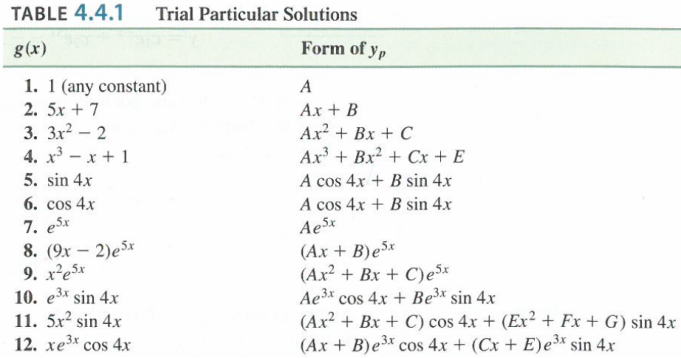
\includegraphics[width=0.95\textwidth]{figs/yptable.pdf}
\end{minipage}
\begin{minipage}[t]{0.4\textwidth}
\phantom{foo}

Mass-spring-damper equivalent forms:
\begin{gather*}
m \frac{d^2x}{dt^2} = -kx -\beta \frac{dx}{dt} \\
\iff \quad m x'' + \beta x' + k x = 0 \\
\iff \quad x'' + 2\lambda x' + \omega^2 x = 0
\end{gather*}
where \quad $\ds\omega = \sqrt{\frac{k}{m}}$, \quad $\ds\lambda = \frac{\beta}{2m}$
\end{minipage}

\bigskip
Converting from $x(t) = c_1 \cos(\omega t) + c_2 \sin(\omega t)$ to $x(t) = A \sin(\omega t + \phi)$:
	$$A = \sqrt{c_1^2 + c_2^2}, \qquad \tan\phi = \frac{c_1}{c_2}$$

\end{document}
